% Chapter Template

\chapter{IoT Healthcare} % Main chapter title

\label{IoT Healthcare} % Change X to a consecutive number; for referencing this chapter elsewhere, use \ref{ChapterX}

%----------------------------------------------------------------------------------------
%	SECTION 1
%----------------------------------------------------------------------------------------
\section{Wearable Devices}
Nowadays, internet connectivity is ubiquitous and has given birth to a whole new
paradigm—The Internet of Things (IoT), namely the concept of interconnecting
physical objects to each other or to the internet to create domain-specific intelli-
gence through seamless pervasive sensing, data analytics and information visual-
ization with cloud computing. Over the years, as we moved from basic internet
services to social networks to wearable web, the demand for interconnecting smart
wearables has increased
\newline

The Google search trend confirms that there is the concurrent growth and
popularity of wearable technology and IoT over the past few years. This presence of
wearable sensor devices is giving a new way to IoT by creating an intelligent fabric
of wearable device or it can be kept near by the body sensors communicating with
each other or with the internet. In other words, Wearable IoT (WIoT) can be defined
as a technological infrastructure that interconnects wearable technology such as
Bluetooth, used to exchange data with wearable sensors, and of heterogeneous
networks, such as WIFI and GSM, used to send the data to the cloud.(Yesha Bhatt and Chintan Bhatt, 2017)

\section{Internet of Things for Personalized HealthCare}
This description initially demonstrates on consumer centric and architectural
requirements for IoT based smarter, connected and personalized healthcare services.
These requirements are then translated into a functional architecture and a mapping
of its components on physical infrastructure is provided.
\begin{itemize}
\item The first requirement of personalized healthcare architecture is availability and
integration of a data generation subsystem from where the physical parameters
will be collected.
\item  The overall architecture system requires a processing and storage system since
the data generating devices cannot support these functionalities due to limited
resources.
\item  The processing and storage system should be able to access the data generation
system regardless of communication technologies used in a network subsystem.
\item  The architecture also requires a consumer subsystem which will receive the
personalized healthcare solutions.
\item  The consumer subsystem should support resource discovery to discover M2M
devices present at data generation subsystem and select appropriate ones for data
collection.
\item  A device management framework is necessary to keep track of the registered
devices and their configurations.
\item  The processing and storage subsystem must incorporate mechanisms for gen-
erating high level abstraction from raw data. This forms the stepping stone for
smarter, connected and personalized healthcare.
\item  Depending on the consumer’s demand, the processing and storage subsystem
should be able to communicate raw data or processed data (high level
abstraction).
\item  The interaction between the mentioned subsystems should occur in a stateless
manner using RESTful principles.
\item  Proper access control policies should be enforced to allow authorized users avail
the personalized healthcare solutions.
\item  The overall system should be able to provide subscription service for occurrence
of a list of events which is notified using push notification.
\end{itemize}

\section{Internet of Things Architecture}
The architecture of IoT consists of several technologies suites to support the IoT. It
demonstrates the integrated technologies related to each other to develop the IoT
system modularity and scalability in different scenarios. The layers’ functionality in
the IoT system as reported in depicted that the IoT architecture consists of
several layers, namely:
\begin{itemize}
\item   Sensor layer which isthelowestlayer consistingof integrated smartobjectsalong
withthesensors.Thesesensorsempowertheinterconnectionofthereal-worldand
the physical measurements for real-time information process. There are a variety
ofsensorswhereeachisusedwithdifferentpurposes.Thesensorscanmeasureair
quality, temperature, electricity and movement. In addition, sensors can have a
memory to record a definite number of measurements.
A sensor can measure a physical property for further conversion into understood
able signal. Most sensors entail connectivity to the sensor gateways (aggrega-
tors) in the form of personal area network (PAN), such as Bluetooth, ZigBee,
and Ultra-Wideband (UWB) or a local area network (LAN), and including WiFi
and Ethernet connections. The wireless sensor networks (WSNs) represents
sensors using low data rate connectivity and low power that form networks.
\item   Gateways and networks layer, where huge data volume is produced by tiny
sensors, which requires a high performance and robust and wired/wireless
network infrastructure. Such networks tied with different protocols to support
machine-to-machine (M2M) networks and their applications. Recently, multiple
networks with several access protocols and technologies are compulsory to
integrate in a heterogeneous configuration.
These networks can be public, private or hybrid models to support the com-
munication requests for bandwidth, latency, or security. Converged network
layer abstraction tolerates multiple hospitals and/or medical centers to share
independently for their routed information without compromising their security,
privacy and performance requirements. Each medical organization in the
healthcare applications utilizes the network as if it is a private network.
\item   Management service layer includes information processing through security
controls, analytics, and devices management. Various analytics methods are
employed to extract applicable information from huge amount of raw data for
processing in faster rate. Furthermore, data-in-motion analysis namely streaming
analytics is obligatory to be executed in real time. Analytics reduces the
network layer stress, and decreases the sensors’ power requirements by less
recurrent communication for faster responses to data established by the sensors.
During data management, the information can be accessed, controlled and
integrated. In addition, data filtering methods including data integration, data
anonymisation, and data synchronization are applied for details hiding for the
information. Data abstraction is applied to extract information to achieve greater
agility and reprocess across domains. Finally, security should be performed
across the whole IoT architecture dimensions. Security is applied to protect the
Internet of Things Driven Connected Healthcare 5
data travels across the whole system. Data integrity enables authentic and
reliable decisions as it inhibits the IoT system unauthorized personnel or
hacking. Researchers were interested to develop several security algorithms as
depicted in . Moreover, various authentication and encryption tech-
nologies for privacy and security using Message Authentication Code
(MAC) and Rivest Shamir Adleman (RSA) guard the transaction data authen-
ticity and confidentiality while transmission between networks. In addition, an
authentication framework that used to support multiple authentication methods
is the Extensible Authentication Protocol (EAP).
For data privacy, technical implementations and policy approaches are engaged
to ensure the removal of the data sensitive. The European Network and
Information Security Agency (ENISA) proposed data privacy approach using
data masking platform to guarantee data privacy. Using IoT-distributed systems
that include embedded devices in public areas, threats produced from other
networks attempts to spoof data access, thus IoT security has to be realized on a
robust foundation at numerous interacting layers.
\item   Application layer includes the various applications of the IoT systems.
\end{itemize}
This IoT architecture is illustrated into layers using various technologies that can
be classified into: (i) technologies concerned with network sharing, latency and
capacity including software-defined radios and cognitive networks, (ii) technologies
influences the microprocessor chips and devices, such as low power sensors and
wireless sensor network, and (iii) services management to sustenance IoT appli-
cations such as in-memory and streaming analytics.(Nilanjan Dey, Amira S. Ashour and Chintan Bhatt, 2017)
\section{About the application}

This application is a proof of concept for a healthcare platform which aims for collecting all the data from different type of devices at this moment the only supported device is a smart band but can be easily extended.

\subsection{Views}

\subsubsection{Smart Bands}
Here you can manage the smart bands registered in this platform and also add new bands. At this moment I support a single type from a single vendor, so the only info needed for managing the bands is the mac address. In the future, I will need more fields like OEM name, the capability of the device: gyroscope, heartbeat sensor, body temperature,  outside temperature, etc.
\begin{figure}[h!]
	\centering
	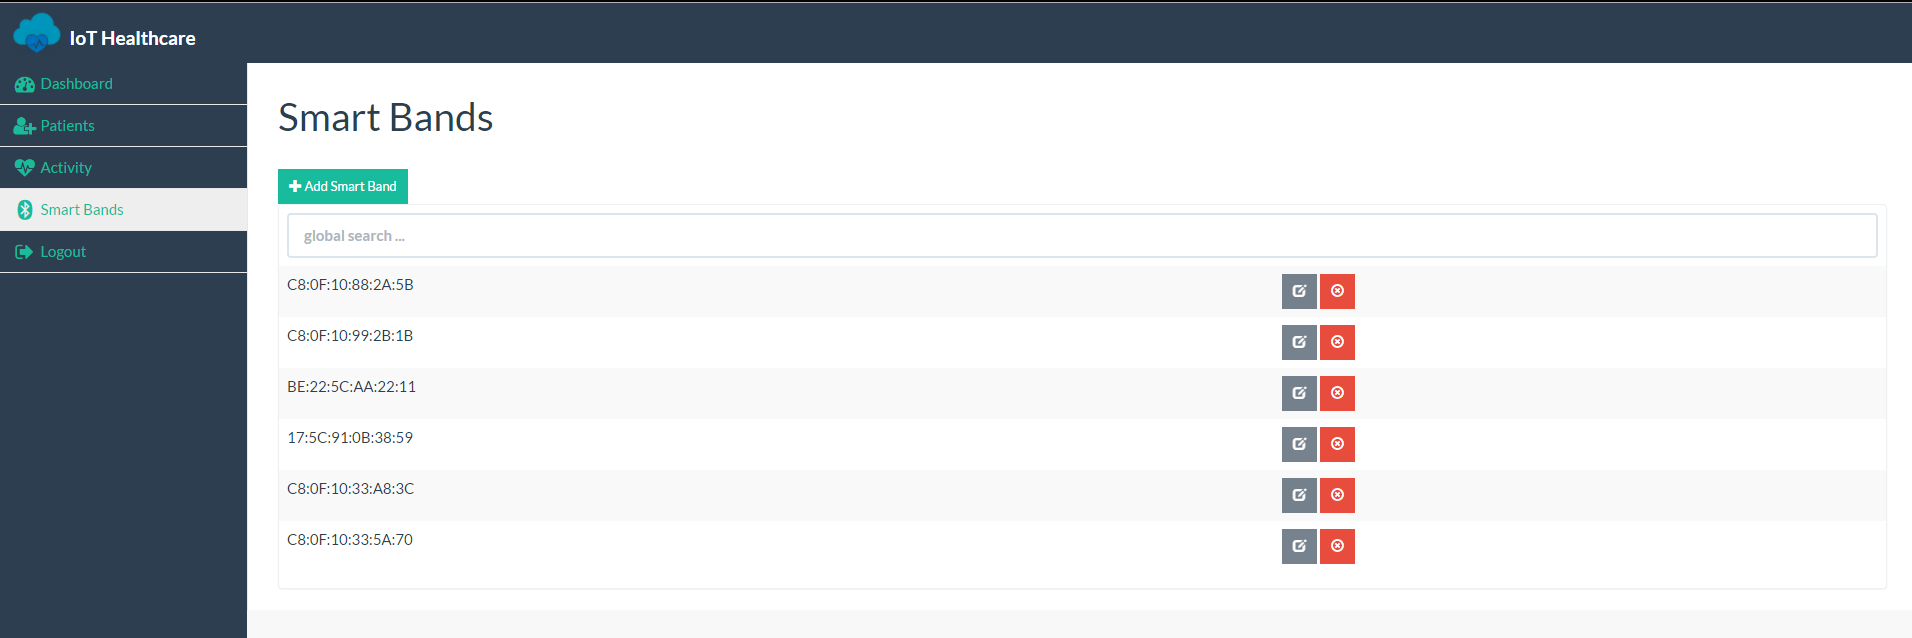
\includegraphics[width=1\textwidth]{./images/iothsmartbands}
	\rule{1\textwidth}{1pt}
	\caption{IoT Healthcare smartbands page}
\end{figure}


\subsubsection{Patients}
In the patients page you can manage all the patients, each patient can have linked a specific smart band.

\begin{figure}[h!]
	\centering
	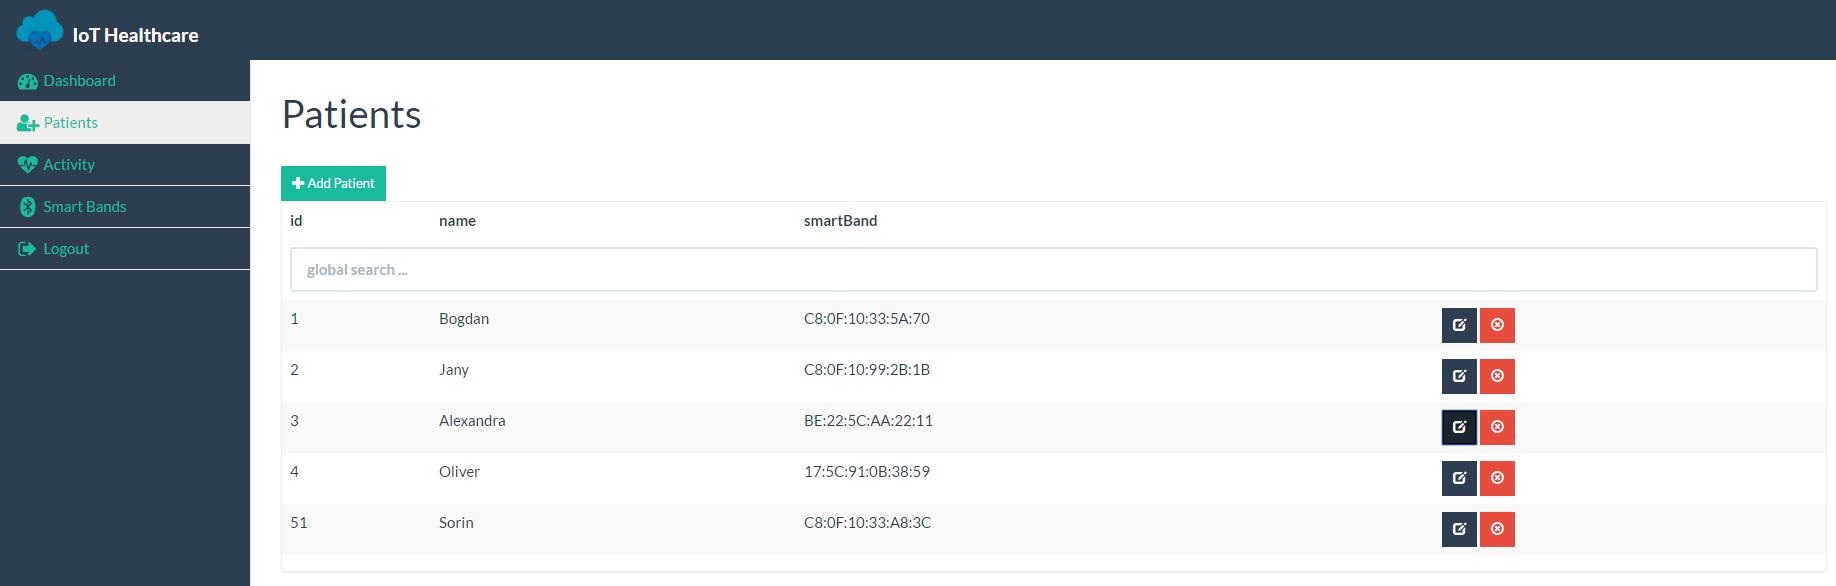
\includegraphics[width=1\textwidth]{./images/iothpatient}
	\rule{1\textwidth}{1pt}
	\caption{IoT Healthcare patients page}
\end{figure}

\subsubsection{Activity}
In the activity tab here is where the magic is happening. The daemon is sending an activity record every 20 min for each patient the record object has the number steps, an array of the heart rate values, the mac address of the smartband and of course the timestamp. 
\newline

\begin{lstlisting}[language=Bash] 
{
	"steps": 500,
	"heartRate": [
		43,
		89,
		30,
		40,
		0,
		5
	],
	"smartBand": {
		"mac": "C8:0F:10:88:2A:5B"
	},
	"timestamp": 1492617449907   
}
\end{lstlisting}      

\begin{figure}[h!]
	\centering
	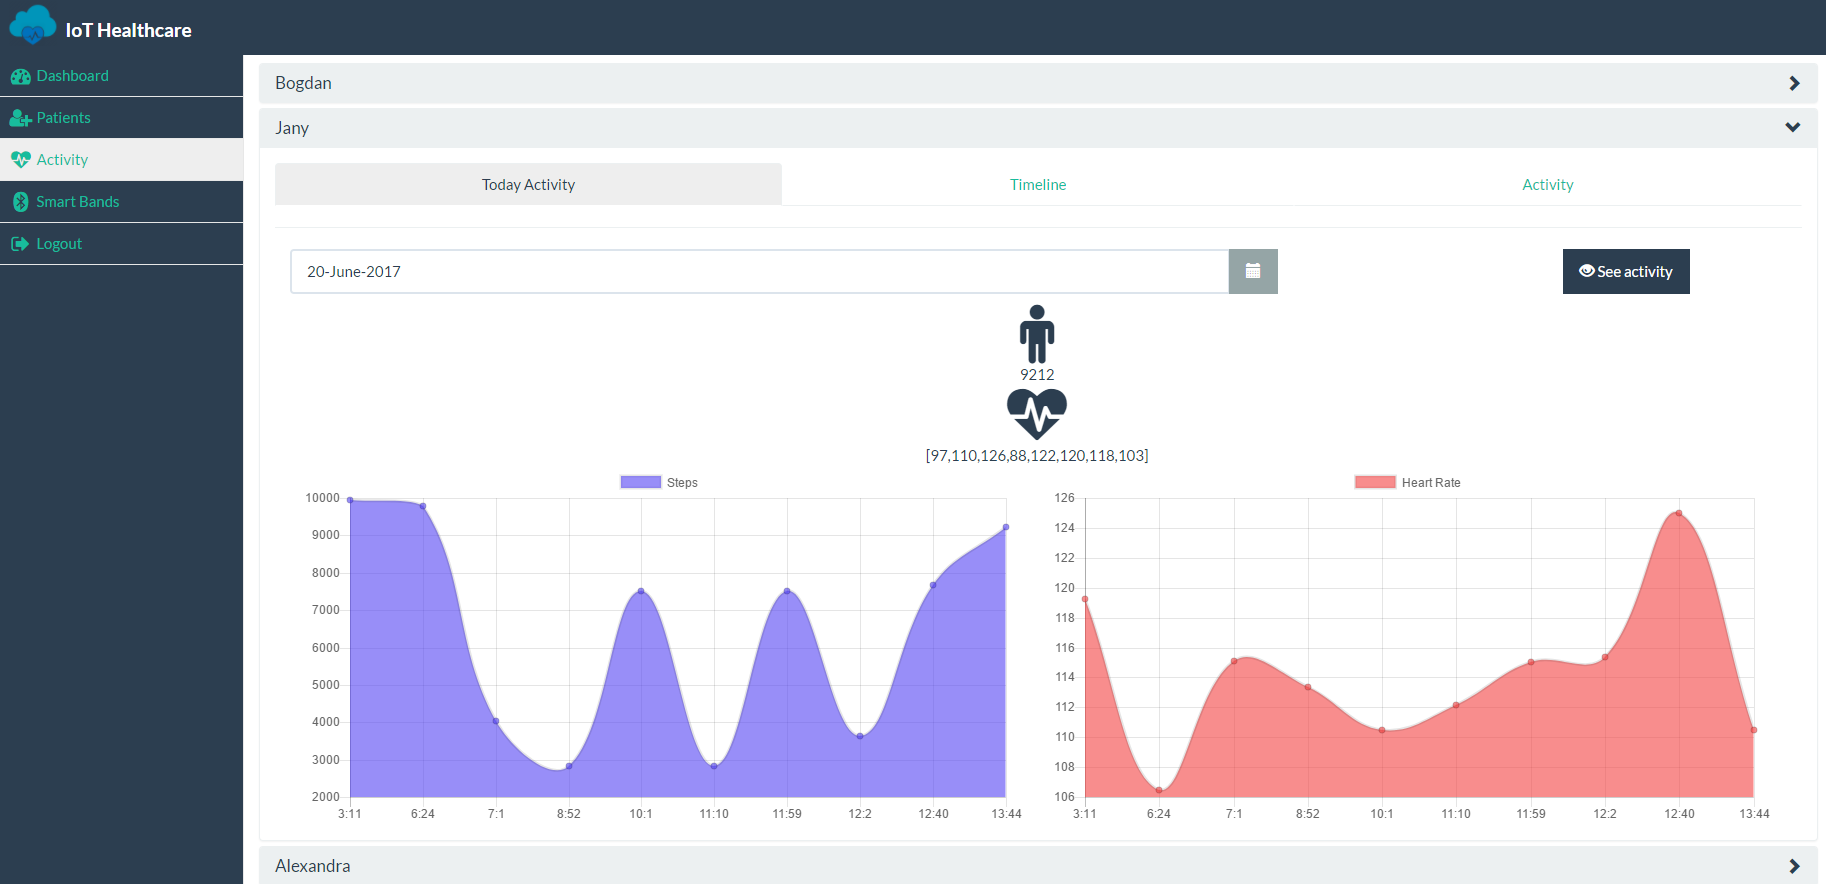
\includegraphics[width=1\textwidth]{./images/iothactivity}
	\rule{1\textwidth}{1pt}
	\caption{IoT Healthcare activity page}
\end{figure}

\section{Challenges and Future Perspectives}
The Internet of Things changed our society anywhere and anytime. Over fast secure
and reliable networks, personalized healthcare and monitoring. Recently, the
standard web services is the most extensively adopted technology for the Internet.
At the network edge, the wireless perceptible embedded healthcare systems requires
functionalities which is challenging in the internet future. Ubiquitous networks and
wireless sensor networks, where the sensors are controlled and connected by the
embedded systems where services encapsulate the functionality and offer unified
access to the system functionality. These components process information in sev-
eral healthcare environments such as households, hospitals, and work as well as it
lead to big data.
\newline
In future, innovative technologies and standards should address privacy and
security features for network, users, data and applications. For network protocol
security, the IPv6 (Internet Protocol Version 6) is the next generation protocol for
the Internet. This protocol encompasses security control and addressing information
to route packets through the Internet.
\newline

With IPv6, IPSec sustenance is integrated into the protocol connections and
design that can be protected/secured when communicating with other IPv6 devices.
The IPSec offers data integrity, data confidentiality and data authentication at the
network layer. Thus, it offers several security services at the IP layer and above.
Such security services include connectionless integrity, access control, protection,
data authentication, encryption, and traffic flow confidentiality. Other IP-based
security solutions are challenging to perform authenticated key exchanges over the
IPSec protocol for payload secure delivery.(Nilanjan Dey, Amira S. Ashour and Chintan Bhatt, 2017)
\newline

Generally, the most challenging issues includes settling on device capabilities,
security, bridging the gaps between individuals,sensors fabrication and safety.
\section{Conclusions}

The Internet of things (IoT) is one of the most noteworthy technology trends.
Innovations merging in the domains of communication and computing, leads to
smart devices that applied in the IoT which not only user-machine interaction but
also concerns with the approach in which the machines involve with each other.
The IoT revolution in healthcare by this time is underway. As recent use cases are
emerging, thus the IoT technology still addresses the urgent necessity for accessible
and affordable care. Meanwhile, the building blocks of the IoT system for auto-
mated and machine-to-machine communication continue to be conventional.
Service layer addition produces the complete IoT infrastructure. This revolution is
characterized by connectivity solutions and end-to-end processing for IoT-driven
healthcare. 
\newline

The Internet of Things still needs the research in healthcare industry. Because as we
know now many people die due to lack of treatment or delay in treatment. The
Internet of Things aspect in HealthCare industry will bring revolution. It will bring
the services at the lower cost to the user who easily cannot afford big treatments like
cancer cure. With the help of various devices RFID and sensors it is easy to connect
patient with hospital but yet many thins to be considered e.g. interface, connectivity
etc. HealthCare in Internet of Things is yet to be in development phase.(Yesha Bhatt and Chintan Bhatt,2017)
\newline

In conclusion, the purpose of this paper was to present a way in which you can create a healthcare application with minimum costs, that can actually make a difference and improve the quality of life for patients, while also lowering the risk of malpractice in the case of medical staff. It is, unfortunately, a reality the fact that errors occur all the time in the medical field, whether it is caused by a lack of concentration or attention, tiredness or simply overlooking a symptom (like a higher heart rate, shallow breathing, an agitated sleeping pattern). With the help of this application (and other similar technologies), we can take a step further into reducing human error and perfecting techniques, when it comes to medical diagnoses. Thus, the Internet of Things will be a game changer in the healthcare industry. This is illustrated by the numerous applications that have appeared on the market, regarding this domain, but also by the ideas and concepts which will eventually evolve into life saving technology.  